\documentclass[11pt]{article}

\usepackage{aa222-jmlr2e}
\makeatother
\usepackage{pdfpages}
\usepackage{sectsty}
\usepackage{hyperref}
\usepackage{graphicx}
\usepackage{subcaption}
\usepackage{float}
\usepackage{amsmath}
\usepackage{booktabs}
\usepackage{multirow}
\usepackage{pgfplots}
\pgfplotsset{compat=1.18}
\usepackage{xcolor}
\usepackage{natbib}
\bibliographystyle{ieeetr}

% ---------------------------------------------------------------------------
% Author-facing flags (delete or blank these macros before submitting):
%   \TODO    something to check / fill in     \CITE  citation to verify
%   \DIAGRAM a figure to insert (PPM->PNG)
% ---------------------------------------------------------------------------
\newcommand{\TODO}[1]{\textcolor{red}{[\textbf{TODO:} #1]}}
\newcommand{\CITE}[1]{\textcolor{blue}{[\textbf{CITE:} #1]}}
\newcommand{\DIAGRAM}[1]{\textcolor{orange}{[\textbf{DIAGRAM:} #1]}}

\begin{document}

\title{Real-Time Stereo Disparity Estimation on Multiple GPUs:\\
A CUDA + MPI Study of Local Matching and Semi-Global Matching}

\author{%
\begin{center}
\begin{minipage}[t]{0.46\textwidth}\centering
\textbf{Frances Raphael}\\
{\ttfamily fraphael@stanford.edu}\\
\end{minipage}\hfill
\begin{minipage}[t]{0.46\textwidth}\centering
\textbf{Aanya Tashfeen}\\
{\ttfamily aanya@stanford.edu}\\
\end{minipage}
\end{center}
}
\maketitle

\noindent\emph{All figures and tables are collected in the appendix and cited
inline; the inline numbers make the main text self-contained within the page
limit.}

% ===========================================================================
\section{Problem Description}
% ===========================================================================

Stereo vision recovers depth from a \emph{rectified} image pair: for each pixel
$(r,c)$ in the left image $I_L$ we seek the horizontal \emph{disparity} $d$ such
that $I_L(r,c)\approx I_R(r,c-d)$. Since $Z=fB/d$ (focal length $f$, baseline
$B$), a dense disparity map is a dense depth map. The input is a rectified 8-bit
pair of size $H\times W$ and a maximum disparity $D_{\max}$; the output is a
disparity map $D(r,c)\in[0,D_{\max})$ stored as float to hold sub-pixel values.
We assume rectification (purely horizontal search) and non-negative disparity,
the standard Middlebury setting~\cite{scharstein2002}.

Depth feeds obstacle avoidance, mapping, and manipulation, and must run at camera
rate (30--60\,Hz). Dense matching costs $\Theta(H\,W\,D_{\max}(2R{+}1)^2)$ for
patch radius $R$: one $1920\times2560$ frame at $D_{\max}{=}64,R{=}2$ is already
$\sim$16\,GOps. A multi-camera rig at high resolution exceeds a single GPU's
compute and memory budget, so we distribute the image across GPUs with MPI,
shrinking both per-GPU work and per-GPU memory.

\paragraph{Contributions.} This report builds a multi-GPU stereo pipeline and
uses it to study what limits dense matching at scale:
\begin{itemize}\itemsep2pt
\item Three CUDA SAD kernels; the shared-memory variant is $2.0\times$ faster,
and a roofline plus Nsight Compute counters show \emph{why}: SAD is
memory-bound, set by on-chip reuse, not arithmetic (Secs.~\ref{sec:model},
\ref{sec:bottleneck}).
\item A GPU Semi-Global Matching implementation (4/8 paths; SAD or Census data
term) compared head-to-head with local SAD. SGM roughly halves the bad-pixel
rate at full coverage; Census makes matching robust to exposure mismatch that
collapses SAD (Sec.~\ref{sec:variants}).
\item An MPI+CUDA row decomposition with halo exchange that scales SAD to
$3.4\times$ on 4 GPUs, with a communication and Amdahl model that predicts the
observed strong/weak scaling (Secs.~\ref{sec:model},~\ref{sec:scaling}).
\item A \emph{distributed} SGM that preserves the exact optimum via boundary
frontier exchange (byte-identical to single-GPU) but scales worse than SAD,
quantifying how a globally-coupled algorithm resists decomposition
(Sec.~\ref{sec:scaling}).
\end{itemize}

% ===========================================================================
\section{Algorithms and State of the Art}
% ===========================================================================

Dense stereo has four stages~\cite{scharstein2002}: matching cost, cost
aggregation, disparity selection, and refinement; methods differ mainly in
aggregation and selection.

\emph{Local block matching} sums a per-pixel cost over a fixed window and takes
the per-pixel winner (WTA). With the sum-of-absolute-differences (SAD) cost,
\begin{equation}
\label{eq:sad}
\mathrm{SAD}(r,c,d) = \!\!\sum_{|i|\le R,\,|j|\le R}\!\!
\bigl| I_L(r{+}i,c{+}j) - I_R(r{+}i,c{+}j{-}d) \bigr|,
\quad D(r,c)=\arg\min_d \mathrm{SAD}(r,c,d).
\end{equation}
It is fast and embarrassingly parallel but blurs depth edges and fails in
textureless or occluded regions because every pixel is decided independently;
this is OpenCV \texttt{StereoBM}~\cite{opencv}.

\emph{Semi-Global Matching} (SGM)~\cite{hirschmuller2008} approximates a 2D
smoothness energy by summing 1D dynamic-programming problems along several image
directions. Along direction $\mathbf{r}$,
\begin{equation}
\label{eq:sgm}
L_\mathbf{r}(\mathbf{p},d) = C(\mathbf{p},d) + \min\!\bigl(
L_\mathbf{r}(\mathbf{p}{-}\mathbf{r},d),\,
L_\mathbf{r}(\mathbf{p}{-}\mathbf{r},d{\pm}1){+}P_1,\,
{\textstyle\min_k} L_\mathbf{r}(\mathbf{p}{-}\mathbf{r},k){+}P_2\bigr)
- {\textstyle\min_k} L_\mathbf{r}(\mathbf{p}{-}\mathbf{r},k),
\end{equation}
with $P_1$ penalizing $\pm1$ steps (slanted surfaces) and $P_2{>}P_1$ penalizing
jumps (depth edges); the summed cost $S=\sum_\mathbf{r} L_\mathbf{r}$ is
minimized over $d$. SGM is the production accuracy/speed sweet spot (OpenCV
\texttt{StereoSGBM}, NVIDIA VPI~\cite{nvidiavpi}, the GPU library
\texttt{libSGM}~\cite{hernandez2016}), usually with 4 or 8 paths and a
Census-transform cost~\cite{zabih1994}. Deep networks~\cite{chang2018} lead on
accuracy but are out of scope for a CUDA+MPI systems study.

We implement local SAD, two accuracy add-ons (sub-pixel refinement and a
left--right consistency check), and SGM, all on GPU (Sec.~\ref{sec:parallel}).
Crucially, our SGM reuses the \emph{same} SAD window as its data term
$C(\mathbf{p},d)$, so comparing it to local SAD isolates the effect of the
aggregation strategy alone rather than confounding it with a different cost.

% ===========================================================================
\section{Parallelization Strategy (CUDA + MPI)}
\label{sec:parallel}
% ===========================================================================

\emph{CUDA kernels.} Each thread computes one output pixel over all $D_{\max}$
disparities; the design axis is how the heavily reused right-image pixels reach
the ALUs. \texttt{basic} reads patches from global memory (reuse only via L2).
\texttt{smem} has a $16\times16$ block stage the left tile and the wider right
tile $(B{+}2R{+}D_{\max})$ into shared memory once, with coalesced loads and
$\sim$$B^2$ reuse per byte. \texttt{tiled} keeps a per-thread register array
\texttt{sad[64]} and sweeps the window once, reusing each left pixel across all
disparities; it also computes the parabolic sub-pixel minimum for free (the cost
curve is already in registers) and backs the LRC check (a second pass with the
images swapped, rejecting pixels whose left- and right-referenced disparities
differ by more than one). For SGM the cost volume is laid out
\texttt{C[(r*W+c)*D+d]} so the $D$ threads of a block read contiguous memory;
each aggregation kernel launches \textbf{one block per scanline}
($\mathrm{next\_pow2}(D)$ threads) that walks the scanline serially---the
recurrence~\eqref{eq:sgm} is a path dependency---while the independent scanlines
run in parallel across blocks, with a shared-memory tree reduction for the
$\min_k$ term.

\emph{MPI decomposition.} We use a 1-D \textbf{row} decomposition (rank $i$ owns
$\lfloor H/P\rfloor{+}[i{<}H\bmod P]$ rows). Rows beat columns by \emph{halo
asymmetry}: SAD needs $R$ halo rows, but because the search is horizontal a
column split would need $D_{\max}{+}R$ halo columns---$33\times$ larger at
$R{=}2,D_{\max}{=}64$. Communication is therefore three operations:
\texttt{MPI\_Scatterv} (each rank's owned rows out from rank 0),
\texttt{MPI\_Sendrecv} ($R$ halo rows with neighbours, no root), and
\texttt{MPI\_Gatherv} (owned disparity rows back)---replacing the Milestone-4
full-image broadcast. Each rank binds a GPU with
\texttt{cudaSetDevice(rank\,\%\,num\_devices)}; host buffers are page-locked
(\texttt{cudaHostRegister}) and copied with \texttt{cudaMemcpyAsync} for true
DMA. We report the slowest rank's kernel time (\texttt{MPI\_Reduce}/\texttt{MAX}).
Figure~\ref{fig:decomp} summarizes the decomposition and all communication.

\begin{figure}[H]
\centering
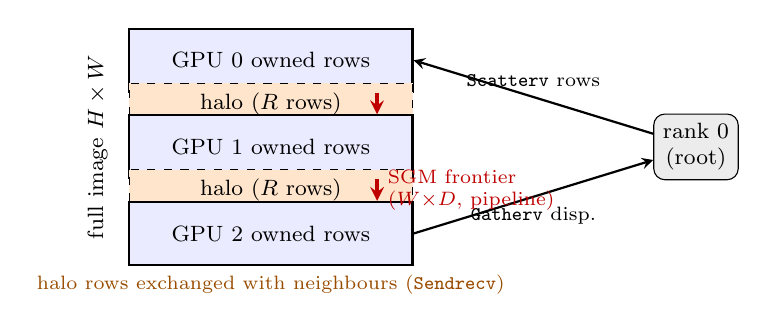
\begin{tikzpicture}[font=\footnotesize, >=stealth,
  slab/.style={draw, thick, minimum width=3.6cm, minimum height=0.8cm, fill=blue!8},
  halo/.style={draw, dashed, minimum width=3.6cm, minimum height=0.26cm, fill=orange!20}]
\node[slab] (s0) at (0,2.6) {GPU 0 owned rows};
\node[halo] (h0) at (0,2.05) {halo ($R$ rows)};
\node[slab] (s1) at (0,1.5) {GPU 1 owned rows};
\node[halo] (h1) at (0,0.95) {halo ($R$ rows)};
\node[slab] (s2) at (0,0.4) {GPU 2 owned rows};
\node[rotate=90] at (-2.2,1.5) {full image $H\times W$};
% root: scatter input rows, gather disparity rows
\node[draw, rounded corners, fill=gray!15, align=center] (root) at (5.4,1.5) {rank 0\\(root)};
\draw[->, thick] (root) -- node[above, font=\scriptsize] {\texttt{Scatterv} rows} (s0.east);
\draw[<-, thick] (root) -- node[below, font=\scriptsize] {\texttt{Gatherv} disp.} (s2.east);
% halo exchange between neighbours (Sendrecv)
\node[font=\scriptsize, orange!60!black, align=center] at (0,-0.25)
  {halo rows exchanged with neighbours (\texttt{Sendrecv})};
% SGM vertical frontier passed down the rank pipeline
\draw[->, very thick, red!75!black] ([xshift=1.35cm]s0.south) -- ([xshift=1.35cm]s1.north);
\draw[->, very thick, red!75!black] ([xshift=1.35cm]s1.south) --
  node[right, font=\scriptsize, red!75!black, align=left] {SGM frontier\\($W{\times}D$, pipeline)} ([xshift=1.35cm]s2.north);
\end{tikzpicture}
\caption{MPI row decomposition (illustrated for 3 GPUs). Each rank owns a slab of
rows plus $R$ halo rows from each neighbour (exchanged with \texttt{Sendrecv});
rank~0 scatters input rows and gathers disparities. Local SAD needs only this.
Distributed SGM additionally pipelines the per-column vertical \emph{frontier}
($W{\times}D$ aggregated costs) from one rank to the next so the semi-global
optimum is preserved across slab boundaries (Sec.~\ref{sec:scaling}).}
\label{fig:decomp}
\end{figure}

% ===========================================================================
\section{Performance Model}
\label{sec:model}
% ===========================================================================

\emph{Roofline}~\cite{williams2009}. Each pixel performs $2(2R{+}1)^2D_{\max}$
integer ops and, with no reuse, loads as many bytes (8-bit pixels), so the naive
operational intensity is $\mathrm{OI}\approx1$\,op/byte. On the Quadro RTX 6000
(672\,GB/s DRAM, $\sim$16.3\,TOps/s) the roofline ridge is $\approx$24\,op/byte,
so SAD is firmly DRAM-bound with a naive ceiling of $\sim$672\,GOps/s. The
falsifiable prediction: performance is set not by arithmetic but by how much
reuse a kernel pulls into the on-chip hierarchy (L2 $\to$ shared memory $\to$
registers).

\emph{Communication ($\alpha+\beta n$)}. Scatter and gather route through rank 0,
which moves $\Theta(HW)$ bytes regardless of $P$ and serializes them, while the
point-to-point halo stays negligible. The model predicts rooted-collective time
that \emph{grows} with $P$ and is the source of strong-scaling loss.

\emph{Amdahl}. Writing $T(P)=T_{\text{comp}}/P+T_{\text{comm}}(P)+T_0$, a larger
image has a smaller serial fraction and must scale better---tested in
Sec.~\ref{sec:scaling}.

% ===========================================================================
\section{Benchmarking, Instrumentation, and Bottlenecks}
\label{sec:bottleneck}
% ===========================================================================

Kernels are timed with CUDA events (mean of 10--20 launches after a warm-up),
MPI phases with \texttt{MPI\_Wtime} barriers, and kernels are profiled in Nsight
Compute. All runs use four Quadro RTX 6000 GPUs on one node.

\emph{Single-GPU kernels} (Table~\ref{tab:kernels}, Fig.~\ref{fig:roofline}).
\texttt{basic} runs at 996\,GOps/s, \texttt{tiled} 1742, \texttt{smem} 2030: the
ordering is set by data reuse, not arithmetic---the memory-bound signature.
\texttt{basic} already exceeds the 672\,GOps/s DRAM ceiling, so its reads are
served from L2; \texttt{smem} wins ($2.0\times$ over \texttt{basic}) by turning
implicit L2 reuse into explicit shared-memory reuse. Nsight Compute
(Table~\ref{tab:ncu}) confirms this directly: \texttt{basic} draws only 0.2\% of
DRAM bandwidth at $\sim$48\% pipe utilization (latency-bound); \texttt{smem}
saturates both compute and memory pipes at 95\% (shared-memory-bound, fastest);
\texttt{tiled} pulls 41\% of DRAM and drops to 69\% occupancy from \texttt{sad[64]}
register pressure. SGM's cost build and aggregation are DRAM-bound (39--67\%) at
low occupancy: SGM materializes the full $H\,W\,D$ cost/accumulator volumes and
streams them five times (one build + four passes), the root of its
$\sim$15$\times$ slowdown versus local SAD.

\emph{MPI phases} (Table~\ref{tab:phases}). The halo exchange is negligible and
constant (0.02--0.04\,ms), validating the row decomposition, while the rooted
scatter+gather grow with $P$ (0.26$\to$3.24\,ms from 1 to 4 ranks) even though
each slab shrinks. As the model predicted, the distributed bottleneck is
root-serialized collective bandwidth---not compute, not halo.

% ===========================================================================
\section{Algorithmic Variants and Their Effect}
\label{sec:variants}
% ===========================================================================

\emph{SAD vs.\ LRC vs.\ SGM} (Table~\ref{tab:accuracy}, Fig.~\ref{fig:qual};
identical SAD data term, scored against Middlebury ground truth). The three are
points on an accuracy/cost/density curve. Local SAD is fastest ($\sim$0.2\,ms)
and dense but error-prone (13--20\% bad pixels). LRC roughly halves the error by
\emph{rejecting} unreliable matches, trading 11--18\% of coverage for
cleanliness. SGM roughly halves the bad-pixel rate \emph{at full coverage}
(tsukuba $20.4{\to}7.4\%$, venus $20.4{\to}9.1\%$) at $4\text{--}6\times$ the cost
of tiled SAD. The deployment choice is dense depth (SGM) versus
sparse-but-trustworthy depth (LRC).

\emph{4 vs.\ 8 paths.} Adding the four diagonal paths nearly doubles SGM runtime
(tsukuba $1.1{\to}2.0$\,ms) for negligible accuracy change ($7.4{\to}7.7\%$ bad)
on these largely fronto-parallel scenes---a clean diminishing-returns variant
that doubles the dominant DRAM traffic without changing the result, so 4 paths is
our default.

\emph{SAD vs.\ Census data term} (Table~\ref{tab:census}). On radiometrically
matched pairs Census is slightly worse than SAD (it discards magnitude). Its
value appears under camera mismatch: scaling the right image by gain 1.4 and bias
15 (different exposure) makes \textbf{every SAD-based method collapse} (tsukuba
$7{\to}87\%$ bad) while \textbf{Census is essentially unchanged}
($12{\to}14\%$), because Census encodes only local intensity \emph{ordering},
which a monotonic gain/bias preserves. For a rig with per-camera auto-exposure
this robustness is decisive.

% ===========================================================================
\section{Scalability Analysis}
\label{sec:scaling}
% ===========================================================================

\emph{Strong scaling} (Table~\ref{tab:strong}, Fig.~\ref{fig:scaling}). The GPU
kernel time scales almost ideally ($3.85\times$/$4.02\times$ at 4 ranks),
confirming balanced compute, but wall speedup is lower ($2.70\times$/$3.42\times$)
because the rooted collectives do not shrink. As Amdahl predicted, the larger
image scales better: 4-rank wall efficiency is 85\% for $1920\times2560$ but 68\%
for $960\times1280$, since the bigger image gives each GPU enough work to amortize
the fixed communication.

\emph{Weak scaling} (480 rows/rank, Fig.~\ref{fig:scaling}). Kernel time is flat
at 0.99\,ms across 1/2/4 ranks (ideal), and wall efficiency stays 91\% at 4
ranks; the only erosion is the $\Theta(P)$ growth of the root collective.
Isoefficiency therefore requires the per-rank slab (not just the total image) to
grow, consistent with the strong-scaling trend.

\emph{Distributed SGM} (Table~\ref{tab:sgmscale}). Under the row decomposition,
SGM's horizontal paths are rank-local but its vertical paths are columns that
cross every boundary. To keep the \emph{global} optimum we pass each rank's
boundary cost row (the ``frontier'', $W\!\times\!D$ ints) to the next rank, which
resumes the recurrence---making the vertical sweep a \textbf{serial pipeline}
across ranks (rank $i$ waits for $i{-}1$). The result is exact (byte-identical to
single-GPU, Sec.~\ref{sec:correct}) but reaches only $1.7\times$/$2.2\times$ at 4
ranks, far below SAD's $2.7\times$/$3.4\times$, despite communication under 12\%.
The gap is \emph{computational}: the vertical pipeline serializes $\sim$40--50\%
of the aggregation. This is the central lesson---global coupling that aids
accuracy fights decomposition: a local method (SAD) distributes embarrassingly, a
semi-global one does not, exactly the Amdahl trade-off from lecture.

% ===========================================================================
\section{Correctness and Verification}
\label{sec:correct}
% ===========================================================================

Against a CPU reference on the synthetic pair ($d^\star{=}24$), integer SAD
reproduces MAE $=0.000$\,px and $0\%$ bad pixels; with sub-pixel the tiled kernel
gives MAE $=0.040$\,px (a harmless fractional residual on integer ground truth)
and still $0\%$ bad. The distributed SAD result is identical on 1, 2, and 4 ranks
(MAE $0.0397$, $0\%$ bad, full coverage), confirming the Scatterv/halo/Gatherv
logic neither drops nor duplicates rows. On real pairs we score against
Middlebury ground truth (Table~\ref{tab:accuracy}; per-dataset disparity scale,
gray~0 = unknown). Finally, distributed SGM is \emph{exact}: its 4-rank output is
byte-identical to the 1-rank output on \texttt{tsukuba} (\texttt{cmp}) and
identical across ranks on synthetic data---any frontier-indexing, pipeline-order,
or halo bug would break the bitwise match.
\TODO{re-paste exact numbers if you re-run, to keep text/tables in sync with
\texttt{results/sgm\_compare.log} and \texttt{sgm\_scaling.csv}.}

% ===========================================================================
\section{Discussion, Limitations, and Future Work}
% ===========================================================================

The biggest payoffs were shared-memory tiling ($2.0\times$, by attacking memory
bandwidth rather than arithmetic) and replacing the full-image broadcast with
\texttt{Scatterv}+\texttt{Sendrecv} (the cheap halo is what lets the large image
hold 85\% efficiency at 4 GPUs). Distributing SGM with frontier exchange was
worth it for the insight: it keeps the exact optimum while exposing the
serial-vertical Amdahl floor. Less worthwhile here: the 8-path diagonals (double
cost, no accuracy gain) and the tiled kernel's fixed 64-slot loop (register
pressure at small $D_{\max}$; a templated bound would help). With more time we
would overlap communication with computation, use CUDA-aware MPI to exchange
frontiers GPU-to-GPU, fuse SGM's four passes to cut its dominant DRAM traffic,
and test a multi-node NVLink/InfiniBand interconnect to see whether the
root-collective bottleneck persists.

% ===========================================================================
\appendix
\section{Detailed Tables and Figures}
\label{app:tables}

\begin{table}[H]
\centering
\caption{Single-GPU SAD kernel variants ($480\times640$, $D_{\max}=64$, $R=2$).}
\label{tab:kernels}
\begin{tabular}{lrrrl}
\toprule
Kernel & Time (ms) & Throughput (GOps/s) & FPS & Reuse mechanism\\
\midrule
\texttt{basic} & 0.875 & \phantom{0}996 & 1143 & L2 cache only \\
\texttt{tiled} & 0.500 & 1742 & 2000 & registers (left-pixel reuse) \\
\texttt{smem}  & 0.429 & 2030 & 2330 & shared memory (tile reuse) \\
\bottomrule
\end{tabular}
\end{table}

\begin{table}[H]
\centering
\caption{Nsight Compute counters (Quadro RTX 6000, $480\times640$, $D_{\max}{=}64$).
SM/Mem = compute/memory-pipe throughput; DRAM = device-memory bandwidth use. The
aggregation row is the horizontal pass (one 64-thread block per scanline).}
\label{tab:ncu}
\begin{tabular}{lrrrrl}
\toprule
Kernel & SM \% & Mem \% & DRAM \% & Occup.\ \% & Limiter\\
\midrule
SAD \texttt{basic} & 46 & 48 & \phantom{0}0.2 & 90 & latency (L2-served)\\
SAD \texttt{smem}  & 95 & 95 & \phantom{0}0.4 & 90 & shared-mem pipe\\
SAD \texttt{tiled} & 44 & 48 & 41 & 69 & DRAM + reg.\ pressure\\
SGM cost-volume    & 17 & 39 & 39 & 80 & DRAM write\\
SGM aggregation    & 46 & 57 & 57 & 41 & DRAM + low occupancy\\
\bottomrule
\end{tabular}
\end{table}

\begin{table}[H]
\centering
\caption{MPI phase times (\texttt{MPI\_Wtime}, weak-scaling config: 480 rows/rank,
$W{=}1280$, $D_{\max}{=}64$). Kernel is the per-rank max.}
\label{tab:phases}
\begin{tabular}{rrrrrrr}
\toprule
Ranks & Image & Scatter (ms) & Halo (ms) & Kernel (ms) & Gather (ms) & Comm \% \\
\midrule
1 & $480{\times}1280$  & 0.056 & 0.000 & 0.987 & 0.201 & --- \\
2 & $960{\times}1280$  & 0.687 & 0.021 & 0.991 & 0.575 & \phantom{0}5.0\% \\
4 & $1920{\times}1280$ & 1.812 & 0.042 & 0.990 & 1.383 & 10.5\% \\
\bottomrule
\end{tabular}
\end{table}

\begin{table}[H]
\centering
\caption{Local SAD vs.\ SAD+LRC vs.\ 4-path SGM on Middlebury (single GPU,
$R{=}2$). ``bad'' = \% pixels with $|{\rm err}|>1$\,px.}
\label{tab:accuracy}
\begin{tabular}{llrrrr}
\toprule
Scene ($D_{\max}$) & Method & MAE (px) & bad (\%) & Coverage (\%) & Time (ms)\\
\midrule
\multirow{3}{*}{tsukuba (16)}
 & SAD (tiled)  & 0.96 & 20.4 & 100.0 & 0.22\\
 & SAD + LRC    & 0.64 & 12.8 & \phantom{0}83.6 & 0.39\\
 & SGM (4-path) & \textbf{0.48} & \textbf{7.4} & 100.0 & 0.88\\
\midrule
\multirow{3}{*}{sawtooth (20)}
 & SAD (tiled)  & 1.25 & 13.3 & 100.0 & 0.22\\
 & SAD + LRC    & \textbf{0.61} & \textbf{6.5} & \phantom{0}89.0 & 0.40\\
 & SGM (4-path) & 1.14 & 10.5 & 100.0 & 1.26\\
\midrule
\multirow{3}{*}{venus (20)}
 & SAD (tiled)  & 1.54 & 20.4 & 100.0 & 0.23\\
 & SAD + LRC    & 0.81 & 10.8 & \phantom{0}81.8 & 0.40\\
 & SGM (4-path) & \textbf{0.94} & \textbf{9.1} & 100.0 & 1.26\\
\bottomrule
\end{tabular}
\end{table}

\begin{table}[H]
\centering
\caption{Bad-pixel rate (\%) with a radiometric perturbation of the right image
(gain 1.4, bias 15), 4-path SGM. Census is invariant to the mismatch.}
\label{tab:census}
\begin{tabular}{llrr}
\toprule
Scene & Right image & SGM (SAD) & SGM (Census)\\
\midrule
\multirow{2}{*}{tsukuba} & matched          & \phantom{0}7.4 & 12.0\\
                         & gain 1.4/bias 15 & 87.2 & \textbf{13.6}\\
\midrule
\multirow{2}{*}{venus}   & matched          & \phantom{0}9.1 & 10.7\\
                         & gain 1.4/bias 15 & 91.5 & \textbf{10.7}\\
\bottomrule
\end{tabular}
\end{table}

\begin{table}[H]
\centering
\caption{Strong scaling of local SAD ($D_{\max}{=}64$, $R{=}2$, 4$\times$RTX 6000).
Speedup/efficiency use wall time.}
\label{tab:strong}
\begin{tabular}{rrrrrrr}
\toprule
Image & Ranks & Kernel (ms) & Wall (ms) & Comm (ms) & Speedup & Eff.\\
\midrule
\multirow{3}{*}{$960\times1280$}
 & 1 & 1.944 & 44.44 & 0.53 & 1.00 & 100\%\\
 & 2 & 0.991 & 24.65 & 1.29 & 1.80 & \phantom{0}90\%\\
 & 4 & 0.505 & 16.43 & 2.17 & 2.70 & \phantom{0}68\%\\
\midrule
\multirow{3}{*}{$1920\times2560$}
 & 1 & 7.907 & 172.98 & 4.29 & 1.00 & 100\%\\
 & 2 & 3.959 & \phantom{0}89.50 & 5.45 & 1.93 & \phantom{0}97\%\\
 & 4 & 1.967 & \phantom{0}50.64 & 6.58 & 3.42 & \phantom{0}85\%\\
\bottomrule
\end{tabular}
\end{table}

\begin{table}[H]
\centering
\caption{Strong scaling of distributed 4-path SGM ($D_{\max}{=}64$, $R{=}2$,
4$\times$RTX 6000); contrast with SAD in Table~\ref{tab:strong}.}
\label{tab:sgmscale}
\begin{tabular}{rrrrr}
\toprule
Image & Ranks & Wall (ms) & Speedup & Eff.\\
\midrule
\multirow{3}{*}{$960\times1280$}
 & 1 & \phantom{0}33.6 & 1.00 & 100\%\\
 & 2 & \phantom{0}23.5 & 1.43 & \phantom{0}71\%\\
 & 4 & \phantom{0}19.6 & 1.71 & \phantom{0}43\%\\
\midrule
\multirow{3}{*}{$1920\times2560$}
 & 1 & 113.9 & 1.00 & 100\%\\
 & 2 & \phantom{0}72.5 & 1.57 & \phantom{0}79\%\\
 & 4 & \phantom{0}52.5 & 2.17 & \phantom{0}54\%\\
\bottomrule
\end{tabular}
\end{table}

\begin{figure}[H]
\centering
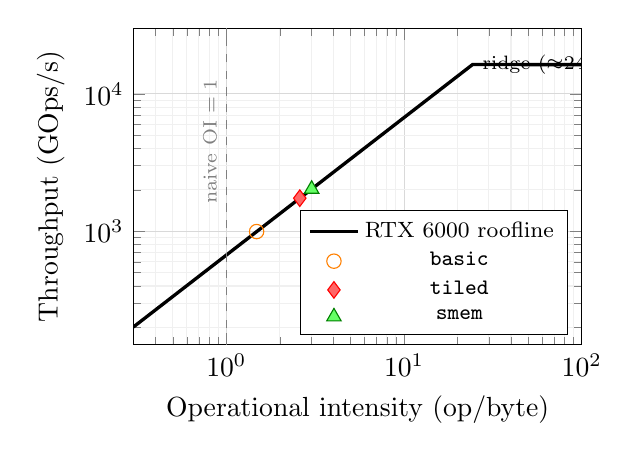
\begin{tikzpicture}
\begin{loglogaxis}[
  width=0.6\linewidth, height=5.6cm,
  xlabel={Operational intensity (op/byte)}, ylabel={Throughput (GOps/s)},
  xmin=0.3, xmax=100, ymin=150, ymax=30000,
  legend pos=south east, legend style={font=\footnotesize},
  grid=both, major grid style={gray!30}, minor grid style={gray!12}]
\addplot[black, very thick] coordinates {(0.3,201.6) (24.3,16329.6) (100,16300)};
\draw[dashed, gray] (axis cs:1,150) -- (axis cs:1,30000);
\node[gray, font=\scriptsize, rotate=90, anchor=south] at (axis cs:1,4500) {naive OI $=1$};
\node[font=\scriptsize, anchor=west] at (axis cs:24.3,16329.6) {ridge ($\approx$24)};
\addplot[only marks, mark=o,        mark size=2.6pt, draw=orange] coordinates {(1.48,996)};
\addplot[only marks, mark=diamond*, mark size=3.0pt, draw=red, fill=red!60] coordinates {(2.59,1742)};
\addplot[only marks, mark=triangle*,mark size=3.0pt, draw=green!50!black, fill=green!60] coordinates {(3.02,2030)};
\legend{RTX 6000 roofline, \texttt{basic}, \texttt{tiled}, \texttt{smem}}
\end{loglogaxis}
\end{tikzpicture}
\caption{Roofline for the SAD kernels (RTX 6000, DRAM 672\,GB/s, ridge
$\approx$24\,op/byte). All kernels are far left of the ridge (memory-bound),
plotted at effective intensity $\mathrm{OI}_{\text{eff}}=$ throughput$/$DRAM\,BW;
each optimization extracts more on-chip reuse, pushing the point rightward.}
\label{fig:roofline}
\end{figure}

\begin{figure}[H]
\centering
\begin{subfigure}[t]{0.48\textwidth}
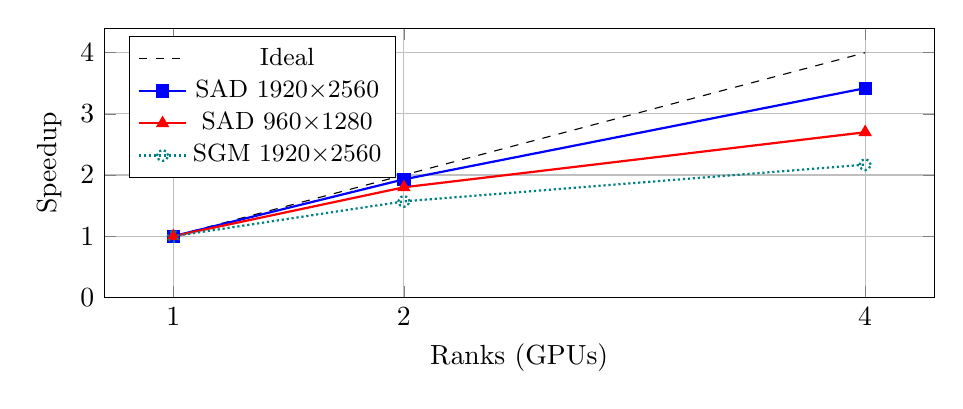
\begin{tikzpicture}
\begin{axis}[width=\linewidth, height=5.0cm, xlabel={Ranks (GPUs)}, ylabel={Speedup},
  xtick={1,2,4}, xmin=0.7, xmax=4.3, ymin=0, ymax=4.4,
  legend pos=north west, legend style={font=\small}, grid=major]
\addplot[black, dashed, domain=1:4, samples=2] {x}; \addlegendentry{Ideal}
\addplot[blue, mark=square*, thick] coordinates {(1,1.00)(2,1.93)(4,3.42)}; \addlegendentry{SAD $1920{\times}2560$}
\addplot[red, mark=triangle*, thick] coordinates {(1,1.00)(2,1.80)(4,2.70)}; \addlegendentry{SAD $960{\times}1280$}
\addplot[teal, mark=o, thick, densely dotted] coordinates {(1,1.00)(2,1.57)(4,2.17)}; \addlegendentry{SGM $1920{\times}2560$}
\end{axis}
\end{tikzpicture}
\caption{Strong-scaling speedup (wall).}
\end{subfigure}\hfill
\begin{subfigure}[t]{0.48\textwidth}
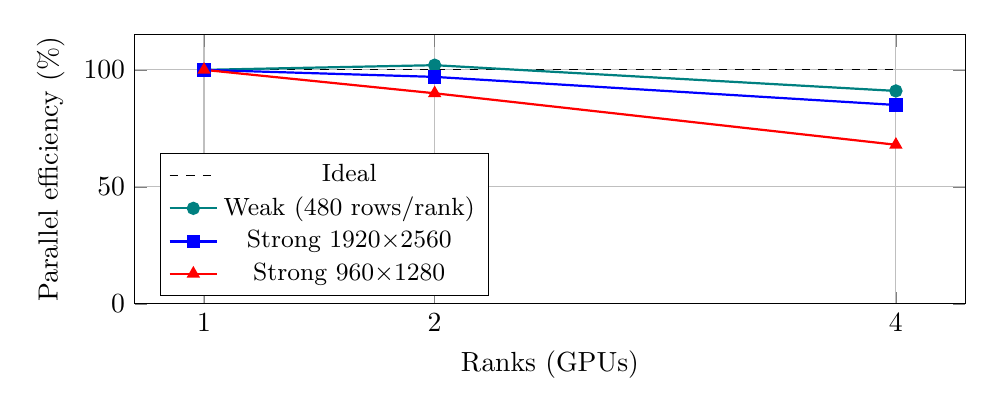
\begin{tikzpicture}
\begin{axis}[width=\linewidth, height=5.0cm, xlabel={Ranks (GPUs)}, ylabel={Parallel efficiency (\%)},
  xtick={1,2,4}, xmin=0.7, xmax=4.3, ymin=0, ymax=115,
  legend pos=south west, legend style={font=\small}, grid=major]
\addplot[black, dashed] coordinates {(1,100)(2,100)(4,100)}; \addlegendentry{Ideal}
\addplot[teal, mark=*, thick] coordinates {(1,100)(2,102)(4,91)}; \addlegendentry{Weak (480 rows/rank)}
\addplot[blue, mark=square*, thick] coordinates {(1,100)(2,97)(4,85)}; \addlegendentry{Strong $1920{\times}2560$}
\addplot[red, mark=triangle*, thick] coordinates {(1,100)(2,90)(4,68)}; \addlegendentry{Strong $960{\times}1280$}
\end{axis}
\end{tikzpicture}
\caption{Parallel efficiency (strong + weak).}
\end{subfigure}
\caption{Scaling on 4$\times$Quadro RTX 6000. SAD compute scales near-ideally;
the wall-clock loss is the rooted scatter/gather. Distributed SGM scales worse
(serial vertical pipeline, Sec.~\ref{sec:scaling}).}
\label{fig:scaling}
\end{figure}

\begin{figure}[H]
\centering
% \DIAGRAM Convert result PPMs to PNG (Python/PIL:
% Image.open('results/tsukuba_sgm.ppm').save('fig/tsukuba_sgm.png')) and
% uncomment this 4-up row (left | ground truth | SAD tiled | SGM):
% \begin{subfigure}{0.24\textwidth}\includegraphics[width=\linewidth]{fig/tsukuba_left.png}\caption{Left}\end{subfigure}\hfill
% \begin{subfigure}{0.24\textwidth}\includegraphics[width=\linewidth]{fig/tsukuba_gt.png}\caption{Ground truth}\end{subfigure}\hfill
% \begin{subfigure}{0.24\textwidth}\includegraphics[width=\linewidth]{fig/tsukuba_tiled.png}\caption{SAD tiled}\end{subfigure}\hfill
% \begin{subfigure}{0.24\textwidth}\includegraphics[width=\linewidth]{fig/tsukuba_sgm.png}\caption{SGM}\end{subfigure}
\fbox{\parbox{0.9\linewidth}{\centering\vspace{0.9cm}
\DIAGRAM{qualitative disparity maps for \texttt{tsukuba} (left, GT, SAD tiled,
SGM) --- PPMs in \texttt{results/tsukuba\_\{gt,tiled,sgm\}.ppm}; convert to PNG
into \texttt{fig/}.}\vspace{0.9cm}}}
\caption{Qualitative comparison: SGM removes the speckle/streaking local SAD
produces in low-texture regions while keeping depth edges sharp.}
\label{fig:qual}
\end{figure}

\section{SGM penalty sweep}
\label{app:sweep}
On \texttt{tsukuba} ($D_{\max}{=}16$) the bad-pixel rate falls monotonically as
$P_1$ rises ($P_1{=}20$: 11.6\%; $P_1{=}80$: 9.3\%; $P_1{=}200,P_2{=}500$: 7.4\%);
penalties have no measurable runtime effect. We fixed $P_1{=}200$, $P_2{=}500$ to
keep $P_2>P_1$ and avoid degenerate over-smoothing (full sweep in
\texttt{results/}).

\section{Reproducibility}
Build with \texttt{make}; all GPU runs go through SLURM on \texttt{gpu-turing}
(no GPU on the login node). Scripts: \texttt{run\_verify\_opt.sh} (SAD
optimizations + accuracy), \texttt{run\_sgm\_final.sh} (SGM vs SAD),
\texttt{run\_sgm\_variants.sh} (4/8-path $\times$ SAD/Census),
\texttt{run\_census\_robust.sh} (radiometric), \texttt{run\_scaling\_final.sh}
(SAD scaling), \texttt{run\_sgm\_dist.sh} (distributed-SGM exactness + scaling),
\texttt{run\_ncu\_profile.sh} (Nsight Compute \texttt{.ncu-rep} reports).
Hardware: one node, 4$\times$Quadro RTX 6000 (Turing, sm\_75, 24\,GB, 672\,GB/s),
NVIDIA HPC SDK (\texttt{nvcc}, \texttt{nvc++}, HPC-X MPI).

\bibliographystyle{ieeetr}
% \TODO verify each entry against the original paper; swap to a .bib if preferred.
\begin{thebibliography}{9}
\bibitem{scharstein2002} D.~Scharstein and R.~Szeliski, ``A taxonomy and
evaluation of dense two-frame stereo correspondence algorithms,'' \emph{IJCV},
47(1--3):7--42, 2002. \CITE{Middlebury taxonomy + dataset}
\bibitem{hirschmuller2008} H.~Hirschm\"uller, ``Stereo processing by
semiglobal matching and mutual information,'' \emph{IEEE TPAMI},
30(2):328--341, 2008. \CITE{original SGM}
\bibitem{zabih1994} R.~Zabih and J.~Woodfill, ``Non-parametric local transforms
for computing visual correspondence,'' \emph{ECCV}, 1994. \CITE{Census transform}
\bibitem{hernandez2016} D.~Hern\'andez-Ju\'arez et al., ``Embedded real-time
stereo estimation via semi-global matching on the GPU,'' \emph{ICCS}, 2016. \CITE{libSGM}
\bibitem{opencv} G.~Bradski, ``The OpenCV Library,'' \emph{Dr.\ Dobb's J.}, 2000. \CITE{OpenCV}
\bibitem{nvidiavpi} NVIDIA, ``VPI: Vision Programming Interface --- Stereo
Disparity,'' developer documentation. \CITE{NVIDIA VPI URL + version}
\bibitem{chang2018} J.-R.~Chang and Y.-S.~Chen, ``Pyramid stereo matching
network,'' \emph{CVPR}, 2018. \CITE{deep-stereo; swap for RAFT-Stereo if preferred}
\bibitem{williams2009} S.~Williams, A.~Waterman, and D.~Patterson, ``Roofline:
an insightful visual performance model for multicore architectures,''
\emph{CACM}, 52(4):65--76, 2009. \CITE{roofline}
\end{thebibliography}

\end{document}
